% Use only LaTeX2e, calling the article.cls class and 12-point type.

\documentclass[12pt]{article}

% Users of the {thebibliography} environment or BibTeX should use the
% scicite.sty package, downloadable from *Science* at
% www.sciencemag.org/about/authors/prep/TeX_help/ .
% This package should properly format in-text
% reference calls and reference-list numbers.

% Use times if you have the font installed; otherwise, comment out the
% following line.
\usepackage{graphicx} 
\usepackage{subfigure}
\usepackage{float}

\usepackage{times}

% The preamble here sets up a lot of new/revised commands and
% environments.  It's annoying, but please do *not* try to strip these
% out into a separate .sty file (which could lead to the loss of some
% information when we convert the file to other formats).  Instead, keep
% them in the preamble of your main LaTeX source file.


% The following parameters seem to provide a reasonable page setup.

\topmargin 0.0cm
\oddsidemargin 0.2cm
\textwidth 16cm 
\textheight 21cm
\footskip 1.0cm


%The next command sets up an environment for the abstract to your paper.



% If your reference list includes text notes as well as references,
% include the following line; otherwise, comment it out.

%\renewcommand\refname{References and Notes}

% The following lines set up an environment for the last note in the
% reference list, which commonly includes acknowledgments of funding,
% help, etc.  It's intended for users of BibTeX or the {thebibliography}
% environment.  Users who are hand-coding their references at the end
% using a list environment such as {enumerate} can simply add another
% item at the end, and it will be numbered automatically.

%\newcounter{lastnote}
%\newenvironment{scilastnote}{%
%\setcounter{lastnote}{\value{enumiv}}%
%\addtocounter{lastnote}{+1}%%
%\begin{list}%
%{%\arabic{lastnote}.}
%{\setlength{\leftmargin}{.22in}}
%{\setlength{\labelsep}{.5em}}}
%{\end{list}}


% Include your paper's title here

\title{Mini-Project Report} 


% Place the author information here.  Please hand-code the contact
% information and notecalls; do *not* use \footnote commands.  Let the
% author contact information appear immediately below the author names
% as shown.  We would also prefer that you don't change the type-size
% settings shown here.

\author
{Xiaotong Li$^{1}$,  Yuchen Yuan$^{2}$ \\
\\
\normalsize{$^{1}$Department of Electrical Eningeering, $^{2}$Department of Computer Engineering}\\
\normalsize{University of California, Santa Cruz}\\
\normalsize{1156 High St, Santa Cruz, CA 95064}\\
\normalsize{Student ID:1634362, 1633572}\\
\normalsize{E-mail:  $\{$xli239, yyuan31$\}$@ucsc.edu.}
}

% Include the date command, but leave its argument blank.

\date{}



%%%%%%%%%%%%%%%%% END OF PREAMBLE %%%%%%%%%%%%%%%%



\begin{document} 

% Double-space the manuscript.

\baselineskip24pt

% Make the title.

\maketitle 



% Place your abstract within the special {sciabstract} environment.



% In setting up this template for *Science* papers, we've used both
% the \section* command and the \paragraph* command for topical
% divisions.  Which you use will of course depend on the type of paper
% you're writing.  Review Articles tend to have displayed headings, for
% which \section* is more appropriate; Research Articles, when they have
% formal topical divisions at all, tend to signal them with bold text
% that runs into the paragraph, for which \paragraph* is the right
% choice.  Either way, use the asterisk (*) modifier, as shown, to
% suppress numbering.

\section*{Introduction}

Mapping high-dimensional data into low-dimensional space through a certain method is a core problem of machine learning and data mining\cite{LargeVis}. The common idea is to express some structures or features of high-dimensional space into low-dimensional space, for example, we will set data points that have similar characteristics together, while the unrelated data points set far apart . The normal dimensionality reduction methods are linear and non-linear. In this mini-project, we mainly try to use three different non-linear methods, t-SNE, LargeVis and TriMap. A non-linear dimensionality reduction method can effectively extract the global features in high-dimensional space. t-SNE was proposed by Maaten and Hinton\cite{t-SNE}. LargeVis was proposed by using the algorithm of knn graph and the stochastic gradient descent for the training process \cite{LargeVis}. TriMap is a dimensionality reduction method that uses triple embedding\cite{TriMap}. We try to use the 60,000 data points dataset Fashion-MNIST which has 10 different classes to experiment and measure the three dimensionality reduction methods using mean precision-recall and trustworthiness-continuity performance.

\section*{Dimensionality Reduction}
In this section, we briefly introduce three dimensionality reduction methods and apply these three methods to the Fashion-MNIST dataset with 10 categories and 60,000 data points. 
\subsection*{t-SNE}
%低维空间
In low-dimensional space, we can define the distribution of data points:
\begin{equation}\label{t-sne low dimensionality}
	q_{ij} = \frac{(1 + ||y_{i}-y_{j}||^2)^{-1}}{\sum_{k\neq l}(1+||y_{k}-y_{l}||^2)^{-1}}
\end{equation}
%高维空间
In high-dimensional space, we can define it this way
\begin{equation}\label{t-sne high dimensionality}
p_{ij} = \frac{p_{j|i}+p_{i|j}}{2n}
\end{equation}
Then we use KL divergence to measure the similarity of this two distribution, and the gradient can be computed as
\begin{equation}\label{t-sne label}
	\frac{\partial C}{\partial y_{i}} = 4 \Sigma_{j}(p_{ij}-q_{ij})(y_{i}-y_{j})(1+||y_{i}-y_{j}||^2)^{-1}
\end{equation}
%所谓的t-SNE算法,总结一下其实就是在SNE的基础上增加了两个改进:一是把SNE变为对称SNE,二是在低维空间中采用了t分布代替原来的高斯分布,高维空间不变。最后来看看t-SNE在可视化效果上是如何完虐其他算法的
This so-called t-SNE algorithm, which is added two improment based on SNE algorithm: Firstly, change original SNE into a symmetric SNE; Secondly, in a low-dimensional space using the t-distribution instead of the original Gaussian distribution, high Dimensional space unchanged.

\subsection*{LargeVis}
%第一步先利用随机投影树得到一个空间划分,在此基础上寻找每个点的k近邻,得到一个初步kNN图,这个kNN图不要求完全准确。第二步根据“邻居的邻居可能也是我的邻居”的思想,利用邻居搜索算法寻找潜在的邻居,计算邻居与当前点、邻居的邻居与当前点的距离并放入一个小根堆之中,取距离最小的k个节点作为k近邻,最终得到一个精确的kNN图。
For LargeVis algorithm, the first step is to use a random projection tree to get a space partition, on the basis of which we find the $k$ nearest-neighbor of each point and get a rough kNN map, which is not required to be completely accurate. The second step is to use the neighbor search algorithm to find potential neighbors and calculate the distance between the neighbors and the current point, then search the neighbors 'neighbors and the current point. Taking the $k$ nodes with the shortest distance as $k$ nearest neighbor, finally it will get an accurate kNN map.
%利用负采样和边采样优化之后,LargeVis还用到了异步随机梯度下降来进行训练,这项技术在稀疏图上是非常有效的,因为不同线程采样的边所连接的两个节点很少有重复的,不同线程之间几乎不会产生冲突。从时间复杂度上来看,每一轮随机梯度下降的时间复杂度为O(sM),其中M是负样本个数,s是低维空间的维数(2或3),随机梯度的步数通常又与点节数量N成正比,因此总的时间复杂度为O(sMN)。从这里可以知道,LargeVis的时间复杂度是与网络中的节点数量呈线性关系的。
LargeVis also uses stochastic gradient descent for training, using negative and edge sampling optimizations. This technique is very efficient on sparse graphs because the two nodes connected by the edges of the different threads are rarely repeated. 
\subsection*{TriMap}
TriMap mainly use a tuple$(i, j, k)$ to represent the relationship with point $i$ and $j$. Different with t-SNE, TriMap use Gaussian similarity function in the high-dimensional space\cite{TriMap}
\begin{equation}\label{TriMap}
	p_{ij}=\rm{exp}(-\frac{||\emph{x}_{\emph{i}}-\emph{x}_{\emph{j}}||^2}{\sigma_{\emph{ij}}^{2}})
\end{equation}
in which $\sigma_{ij}^{2} = \sigma_{i}\sigma_{j}$. For low dimension, it is represented as
\begin{equation}
	q_{ij}=(1+\frac{||y_{i}-y_{j}||^2}{a})^{-\frac{1+\alpha}{2}}
\end{equation}
Then it use two different ways, which is Nearest-neighbors triplets and random triplets to form the  embedding.
\paragraph*{Figure.1} The three graphs below are the results after using three different dimension reduction methods on the Fashion-MNIST dataset\cite{fahionMNIST}.  Each example is a 28$\times$28 grayscale image, associated with a label from 10 classes. The classification of figure (a) looks better and different types of data points were significantly spaced. Data points of figure (b) and (c) in some region will be concentred together. .%上面三个图是在fashionMNIST数据集上使用三种不同的降维方法后的效果图
\begin{figure} [H]
	\subfigure[t-SNE]{
		\label{Fig.sub.2}
		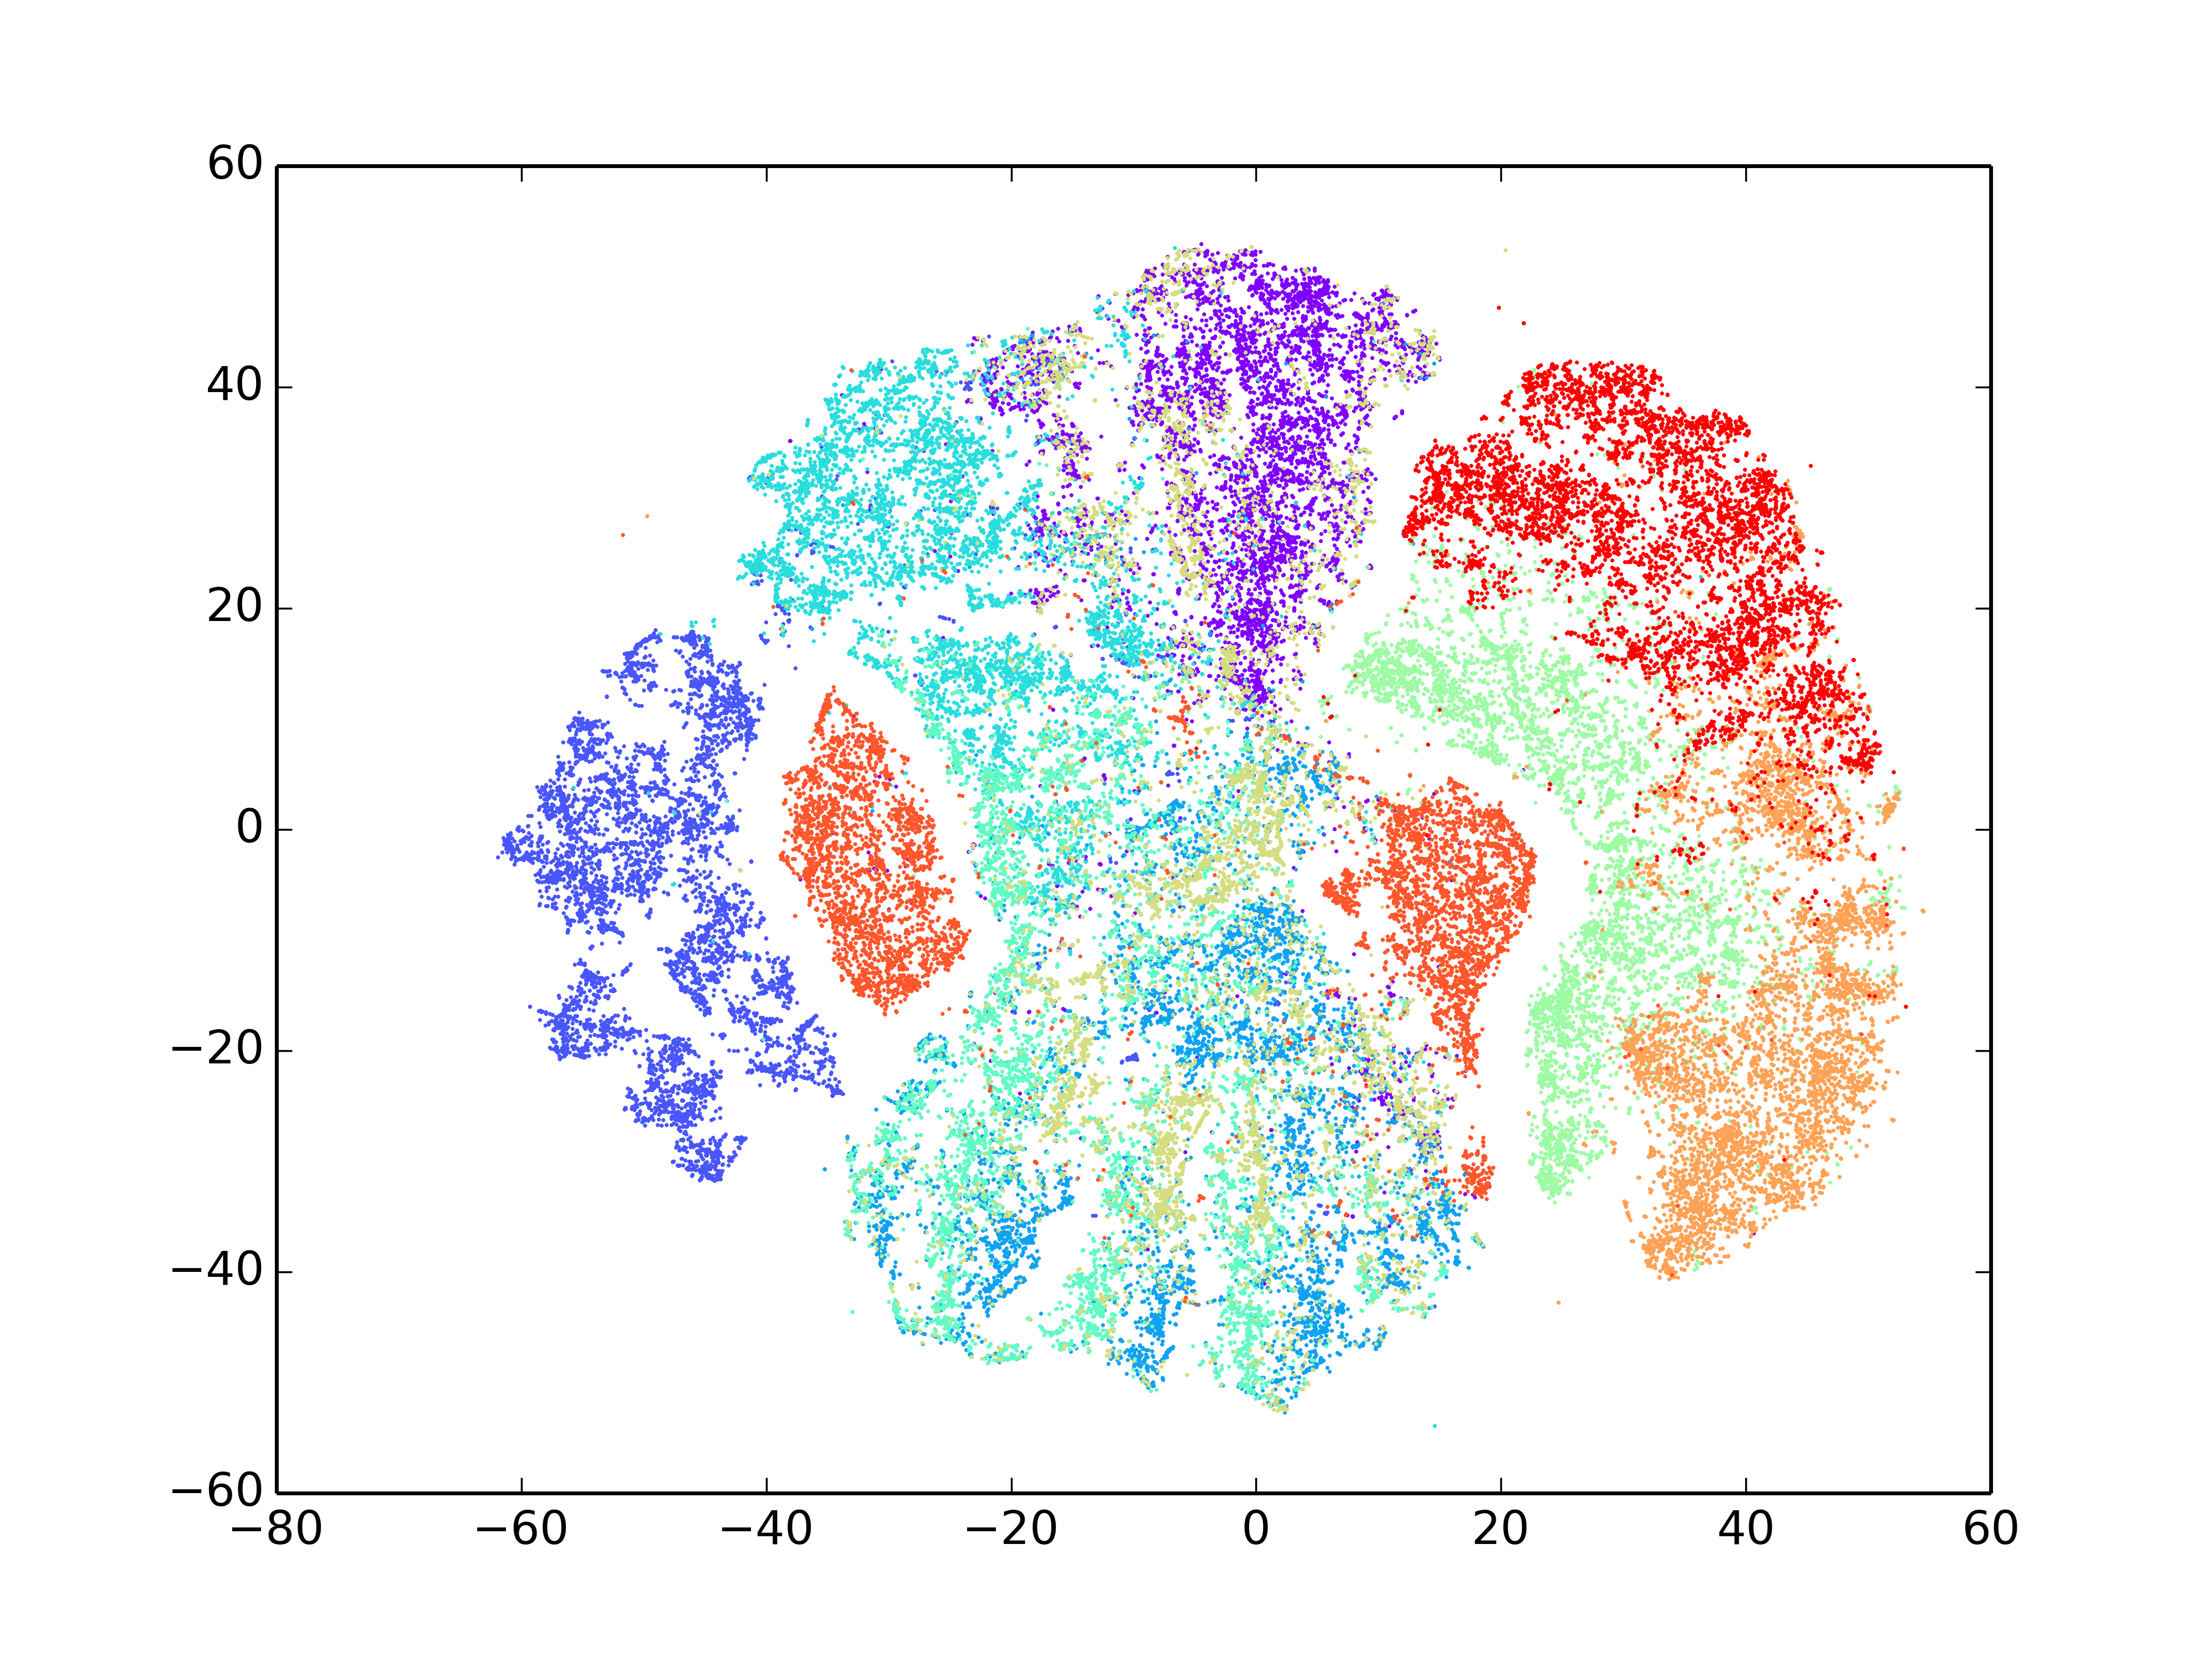
\includegraphics[width=0.47\textwidth]{tsne_plot2D.png}}
	\subfigure[LargeVis]{
		\label{Fig.sub.}
		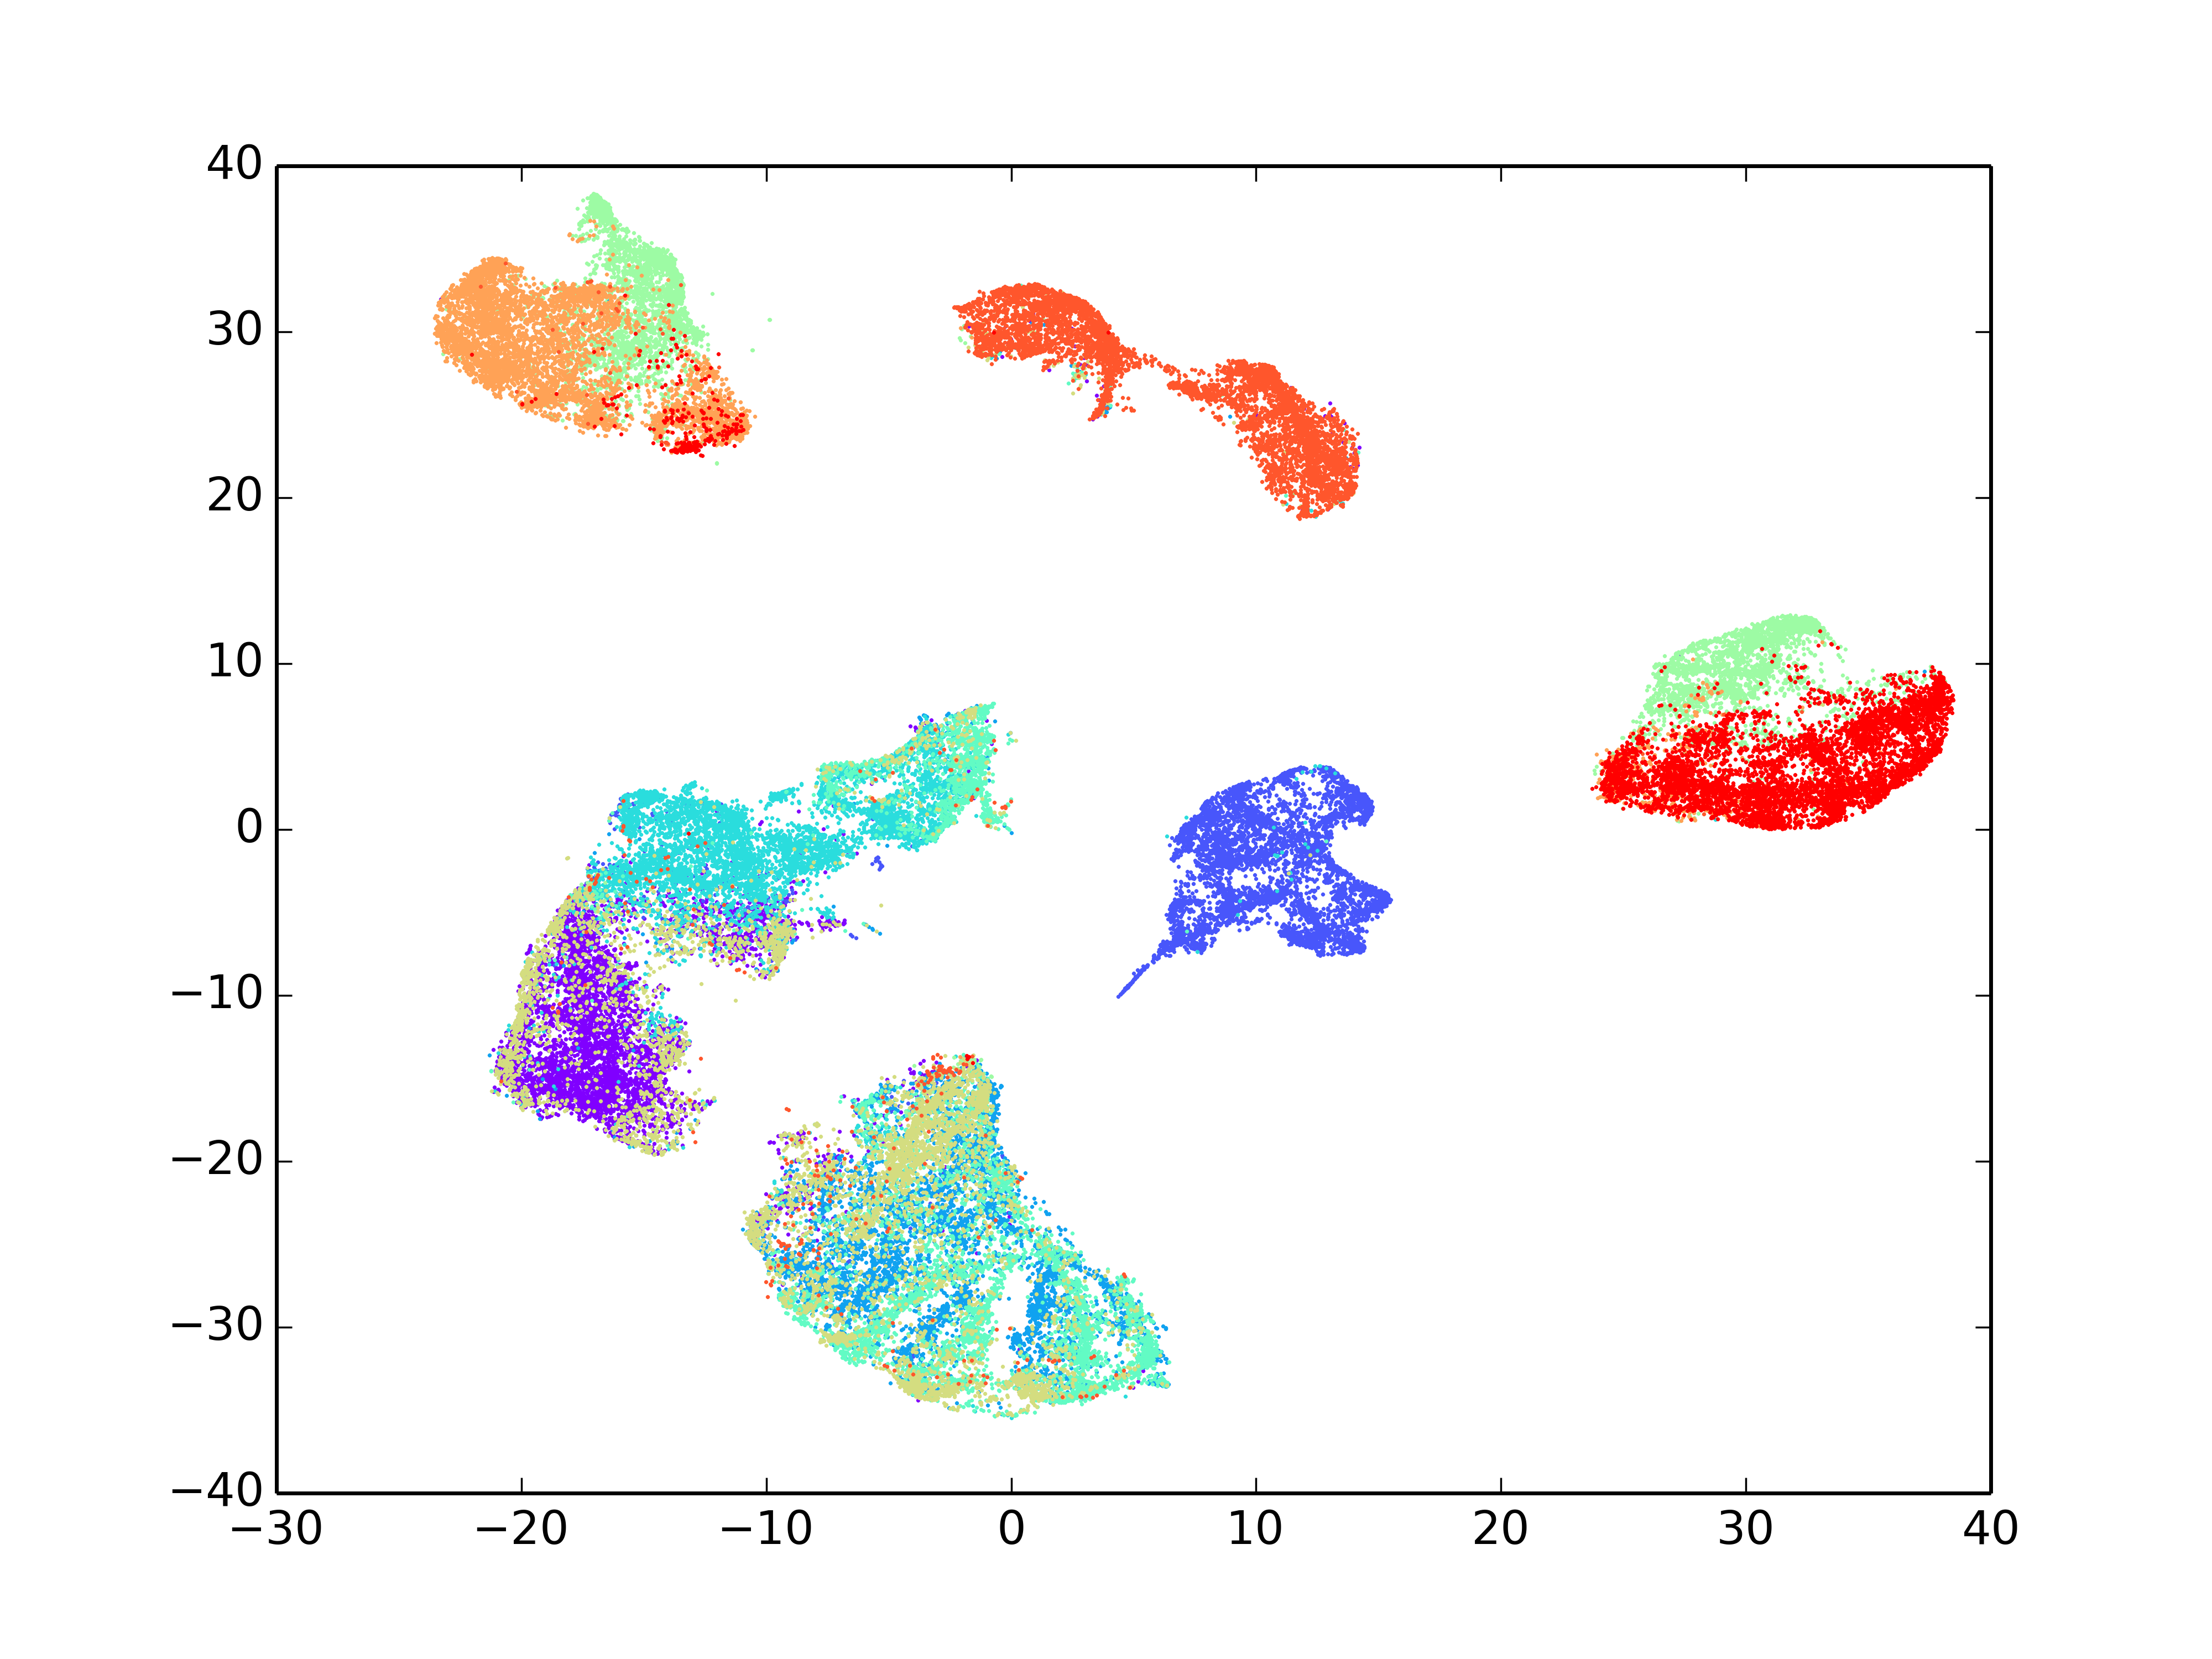
\includegraphics[width=0.47\textwidth]{largeVis_plot2D.png}}
	\centering
	\subfigure[TriMap]{
		\label{Fig.sub.1}
		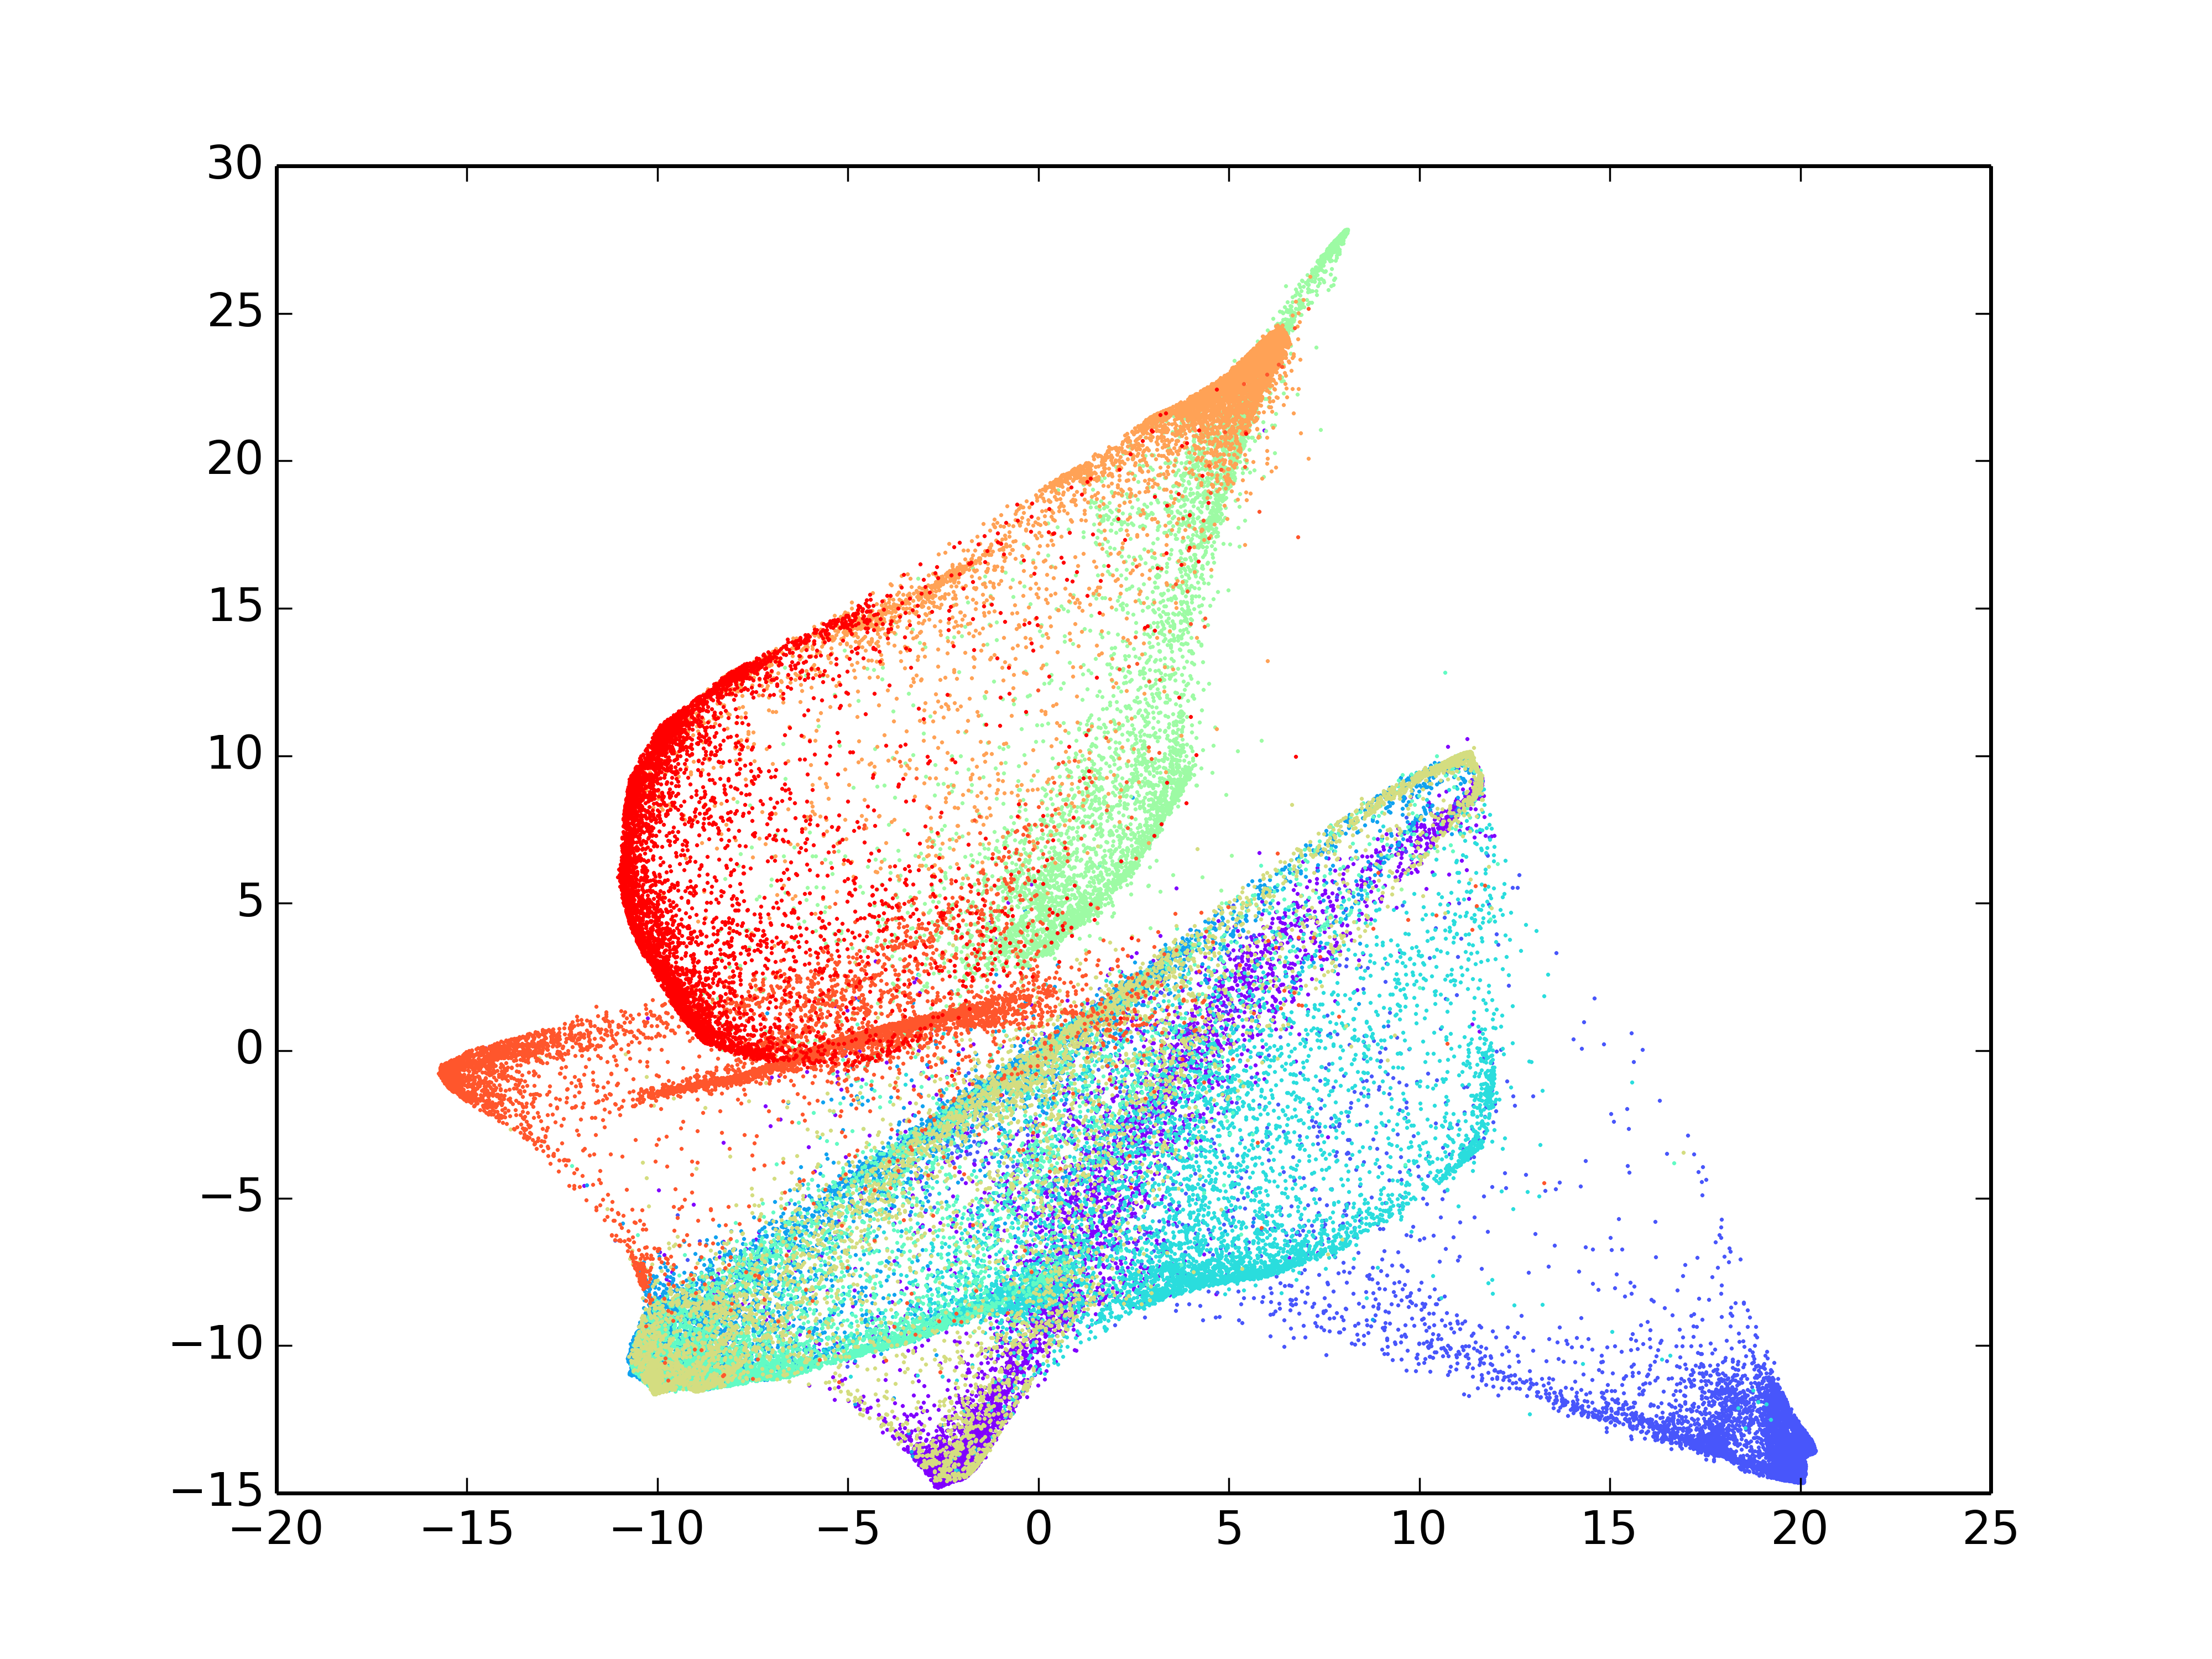
\includegraphics[width=0.47\textwidth]{trimap_plot2D.png}}
	\caption{Dimensionality Reduction}
	\label{Fig.1}
\end{figure}



\section*{Experiment and Quality Evaluate}
In this section, we introduce and apply two tools to measure the effect of dimensionality reduction: mean precision-recall and trustworthiness-continuity. By analyzing these two types of curves, we can evaluate the effect of dimensionality reduction
\subsection*{Mean Precision-Recall}
The paper gives the traditional definition of precision\cite{mean Precision-Recall}:
\begin{equation}
	\rm{Precision}(\emph{i}) = \frac{\emph{N}_{\rm{TP},\emph{i}}}{\emph{k}_{\emph{i}}}
\end{equation}
Which means in low-dimension space, the output point $i$ has $k_{i}$ neighbors. Generally, Number of TP (True Positive) means number of points that both in high-dimension space and in low-dimension space. However, the definition of recall is 
\begin{equation}
	\rm{Recall}(\emph{i}) = \frac{\emph{N}_{\rm{TP}, \emph{i}}}{\emph{r}_{\emph{i}}}
\end{equation}
Here $r_{i}$ means in high-dimension space, the number of neighbors of input point $i$. As we know, the value of $N_{\rm{tp}}$ would change according to the $r_{i}$ and $k_{i}$. To get the precision-recall curve, we fixed $r_{i}$, and change the value of $k_{i}$ to see how the precision and recall value fluctuate.
Our test dataset is MNIST2500, which contains 2500 points and each point has 784 dimension data \cite{MNIST}. Using KNN tool from scikit-learn to get $k$ nearest neighbors of input points and output points depends on given $r$ and $k$, 
We divide our code into 3 parts:
\begin{enumerate}
	\item [(1)]For each point $i$, we calculate the input neighbor with $r=75$, then calculate the output neighbor with $r$ from 1 to 75.
	\item[(2)] For each value of $r$, we compare the same points in low-dimension neighbor and high-dimension, got the value of TP then store.
	\item[(3)] After got 75 precision and recall values, we calculate the mean value of them and plot the curve.
\end{enumerate}


\subsection*{Trustworthiness-Continuity}
It's kindly same to previous paper, firstly, it gives the definition of two terms. Trustworthiness\cite{Trust1}\cite{Trust2},
\begin{equation}
	T(k) = 1-A(k)\sum_{i=1}^{N}\sum_{x_{j}\in U_{k}(x_{i})}(r(x_{i},x_{j})-k)
\end{equation}
let $N$ be the number of data at high-dimension space and $ r(x_{i} , x_{j})$ be the rank of the data sample $x_{j}$ in the ordering according to distance from $x_{i}$ in the original data space. Denote by $U_k(x_{i})$ the set of those data samples that are in neighborhood of sample $x_{i}$ in the low-dimension data space but not in the high-dimension data space. $A(k) = 2/(N\times k (2N - 3k - 1))$ scales the values between zero and one. Similarly, the definition of Continuity is\cite{Trust1}\cite{Trust2}
\begin{equation}
	C(k) = 1-A(k)\sum_{i=1}^{N}\sum_{x_{j}\in V_{k}(x_{i})}(\hat{r}(x_{i},x_{j})-k)
\end{equation}
$r(x_{i} , x_{j} )$ be the rank of the data sample $x_{j}$ in the ordering according to distance from $x_{i}$ in the low-dimension space. $V_k (x_{i})$ be the set of those data samples that are in the neighborhood of the data sample $x_{i}$ in the high-dimension space but not in the low-dimension data space. For the same test dataset MNIST2500 \cite{MNIST}. We still use kNN tool to find nearest neighbor. The difference between previous one is we generate a rank-matrix in both high-dimension space and low-dimension space both.
We divide our code into 5 parts:
\begin{enumerate}
	\item[(1)]According to the high-dimension dataset size, we create the high-rank matrix of $(2500\times2500) $ to store the rank between each pair of points. Same to low-dimension dataset, and low-rank matrix.
	\item[(2)] For each point $ i$, we calculate the input neighbor and output neighbor with $r=k $ from 1 to 75. Because the Trustworthiness and Continuity needs the same $k $ value
	\item[(3)] For each value of $k$ we compare the points in low-dimension neighbor and high-dimension neighbor, got the $U_{k}$ and $V_{k}$.
	\item[(4)] 	For every point in $U_{k}$ , we got the rank value from high-dimension rank matrix, same to every point in $V_{k}$. Then store these rank value.
	\item[(5)] After executing $k=75$, sum all the rank value and put them in the formula, got the final value of Trustworthiness and Continuity.
\end{enumerate}
\hfill


\begin{figure}[H] 
	\subfigure[Continuity]{
		\label{Fig.sub.1}
		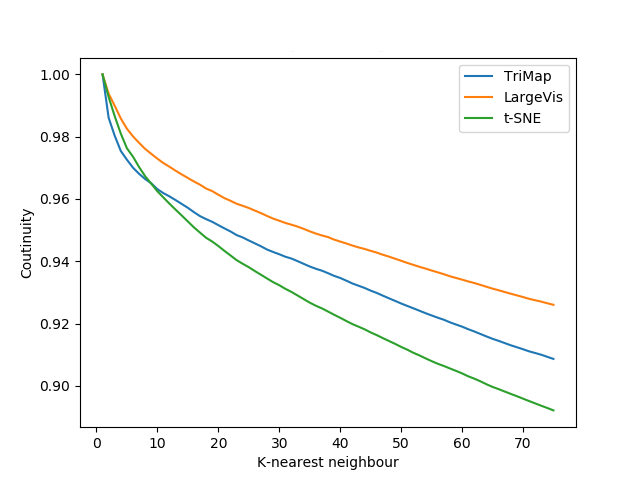
\includegraphics[width=0.47\textwidth]{continuity.png}}
	\subfigure[Trustworthiness]{
		\label{Fig.sub.}
		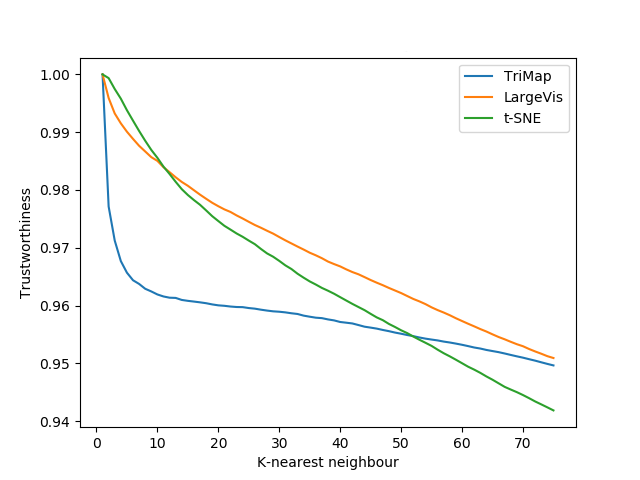
\includegraphics[width=0.47\textwidth]{trustworthiness.png}}
\centering
	\subfigure[Mean Precision-Recall]{
		\label{Fig.sub.2}
		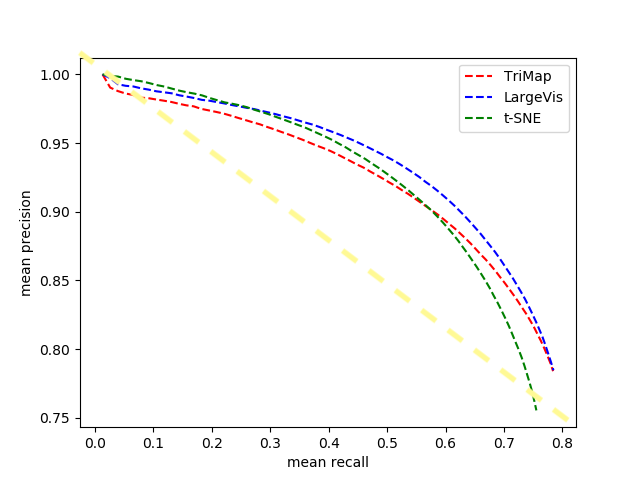
\includegraphics[width=0.47\textwidth]{precision-recall.png}}
	\caption{Quality Measurement}
	\label{Fig.2}
\end{figure}

\paragraph*{Figure.2}
\begin{enumerate}
	\item From the figure (a) we can see that the three methods are relatively smooth curve, when changing the $k$ value, the recall value increases, indicating the predicted point contains more and more correct points, at the same time it contains more other errors, so the precision value reduces. largeVis is closer to (1, 1) points than the other two methods, indicating that the quality is better.
	\item For Trustworthiness, which is figure (b) we find $k$ neareast-neighbors in both high and low dimensions. The TriMap indicated by the blue line decreases very rapidly when the number of neighbors increases in low dimension. When the number of nearest-neighbours is also increasing, However, LargeVis and t-SNE did not change very much due to the growth of $k$, and finally three methods have similar values.
	\item In Continuity figure (c), these three methonds changes similar with the increase of $k$ nearest-neighbour, but TriMap and LargeVis are little better compared with the performance.
\end{enumerate}

\section*{Conclusion}
In this project, we learned and understood three different non-linear dimensionality reduction methods, t-SNE, LargeVis, and TriMap. LargeVis has great advantages when it comes to running large datasets, while TriMap and t-SNEs take a long time to run on computer. At the same time, we measure and analyze the quality of these three methods by implementing mean Precision-Recall and Trustworthiness-Continuity. In trustworthiness, TriMap decreases significantly with he number of $k$ nearest-neighbors increase, and the performance of the other two methods is slightly stable. In the mean-Precision-Recall and Continuity, these three methods performance are similar.


% Your references go at the end of the main text, and before the
% figures.  For this document we've used BibTeX, the .bib file
% scibib.bib, and the .bst file Science.bst.  The package scicite.sty
% was included to format the reference numbers according to *Science*
% style.
\clearpage

\begin{thebibliography}{10}
	\bibitem{LargeVis}Tang, Jian, et al. Visualizing large-scale and high-dimensional data. \emph{Proceedings of the 25th International Conference on World Wide Web}. International World Wide Web Conferences Steering Committee, 2016.
	\bibitem{TriMap}Amid, Ehsan, and Manfred K. Warmuth. \emph{Transformation invariant and outlier revealing dimensionality reduction using triplet embedding.} (2018).
	\bibitem{t-SNE}Maaten, Laurens van der, and Geoffrey Hinton. Visualizing data using t-SNE. \emph{Journal of machine learning research} 9.Nov (2008): 2579-2605.
	\bibitem{mean Precision-Recall}Venna, Jarkko, et al. Information retrieval perspective to nonlinear dimensionality reduction for data visualization. \emph{Journal of Machine Learning Research} 11.Feb (2010): 451-490.
	\bibitem{Trust1}Kaski, Samuel, et al. Trustworthiness and metrics in visualizing similarity of gene expression. \emph{BMC bioinformatics} 4.1 (2003): 48.
	\bibitem{Trust2}Venna, Jarkko, and Samuel Kaski. Local multidimensional scaling with controlled tradeoff between trustworthiness and continuity. \emph{Proceedings of WSOM.}  Vol. 5. 2005.
	\bibitem{fahionMNIST}Xiao, Han, Kashif Rasul, and Roland Vollgraf. Fashion-mnist: a novel image dataset for benchmarking machine learning algorithms. \emph{arXiv preprint} arXiv:1708.07747 (2017).
	\bibitem{MNIST}Yann LeCun, Corinna Cortes, and Christopher JC Burges. The mnist database of handwritten digits, 1998.
\end{thebibliography}


% Following is a new environment, {scilastnote}, that's defined in the
% preamble and that allows authors to add a reference at the end of the
% list that's not signaled in the text; such references are used in
% *Science* for acknowledgments of funding, help, etc.




% For your review copy (i.e., the file you initially send in for
% evaluation), you can use the {figure} environment and the
% \includegraphics command to stream your figures into the text, placing
% all figures at the end.  For the final, revised manuscript for
% acceptance and production, however, PostScript or other graphics
% should not be streamed into your compliled file.  Instead, set
% captions as simple paragraphs (with a \noindent tag), setting them
% off from the rest of the text with a \clearpage as shown  below, and
% submit figures as separate files according to the Art Department's
% instructions.




\end{document}
